\newpage
\usecasebase{Inserimento di \textit{feedback}}
\label{usecase:Inserimento di feedback}

\begin{figure}[h]
	\centering
	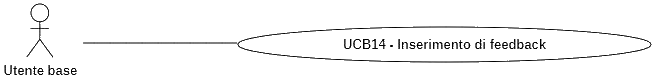
\includegraphics[width=0.8\textwidth]{./uml/UCB14.png} 
	\caption{Inserimento di \textit{feedback}}
	\label{fig:UCB16}
  \end{figure}

\begin{itemize}
	\item \textbf{Attore principale:} Utente base.

	\item \textbf{Precondizione:} 
	\begin{itemize}
		\item L'Utente base ha completato un ordine e lo ha pagato.
		\item L'Utente base si trova nella pagina di dettagli di un ristorante (vedi
		\autoref{usecase:Visualizzazione di un ristorante}) e preme il bottone "Inserisci recensione".
	\end{itemize}

	\item \textbf{Postcondizione:} L'Utente base ha lasciato un \textit{feedback}.

	\item \textbf{Scenario principale:}
	      \begin{enumerate}
		      \item L'Utente base si trova nella pagina adibita per l'inserimento del \textit{feedback} del ristorante;

		      \item L'Utente base compila il \textit{form} del \textit{feedback} del ristorante, inserendo: 
		            \begin{itemize}
			            \item Un testo descrittivo del \textit{feedback};
			            \item Una valutazione da 1 a 10;
		            \end{itemize}

		      \item L'Utente base conferma il \textit{feedback};

		      \item Il Sistema registra il \textit{feedback};

	      \end{enumerate}
\end{itemize}
